\section{Datenbankdesign}
Um die Erweiterung der Datenbank für den Feasibility Check zu erklären, wird zunächst auf die grundlegende Struktur der REALIS-Datenbank eingegangen. In Abbildung \ref{fig:realis-datenbankdesign} ist ein Ausschnitt der wichtigsten Tabellen und deren Beziehungen zueinander dargestellt, einschließlich der vorgenommenen Erweiterungen, die durch orange Rechtecke gekennzeichnet sind. In den folgenden Erläuterungen sind die zugehörigen Tabellennamen aus der Abbildung \ref{fig:realis-datenbankdesign} jeweils in Klammern angegeben.

\subsection{REALIS-Datenbank}

Wie bereits in Kapitel \ref{Subsec:project-lifecycle} beschrieben, besteht ein \textbf{REALIS-Projekt} (\texttt{relproject}), das zur Qualifizierung neuer Produkte dient, aus mehreren \textbf{Tests} (\texttt{test}). Jeder Test besitzt einen eindeutigen \textbf{Status} (\texttt{ctlg\_state\_type}), der zu Beginn auf ''NEW'' gesetzt wird und nach Abschluss den Status ''ARCHIVE'' erhält (vgl. Abbildung \ref{fig:realis-project-lifecycle}, rechte Spalte). Zudem wird jeder Test einer Kategorie bzw. einem \textbf{Test-Typen} (\texttt{ctlg\_\-test\-\_sub\_type}) zugeordnet.

Ein Test besteht aus mehreren aufeinanderfolgenden \textbf{Operationen} (\texttt{operation}), die nacheinander im \gls{RPT}-Labor abgearbeitet werden. Die Tabellen, die eng mit der Operation verknüpft sind, sind in Abbildung \ref{fig:realis-datenbankdesign} im grün umrandeten Bereich dargestellt. Jede Operation kann dabei einen oder mehrere \textbf{Parameter} (\texttt{op\_data}) enthalten, die beispielsweise die Umgebungsbedingungen definieren. Die konkreten Werte dieser Parameter sind in dem Eintrag \texttt{OPD\_PLAN} hinterlegt. Jedem Parameter wird außerdem ein \textbf{Parameter-Typ} (\texttt{ctlg\_op\_\-data\_type}) zugewiesen.  


\begin{figure}[!htbp]
    \centering
    \makebox[\textwidth]{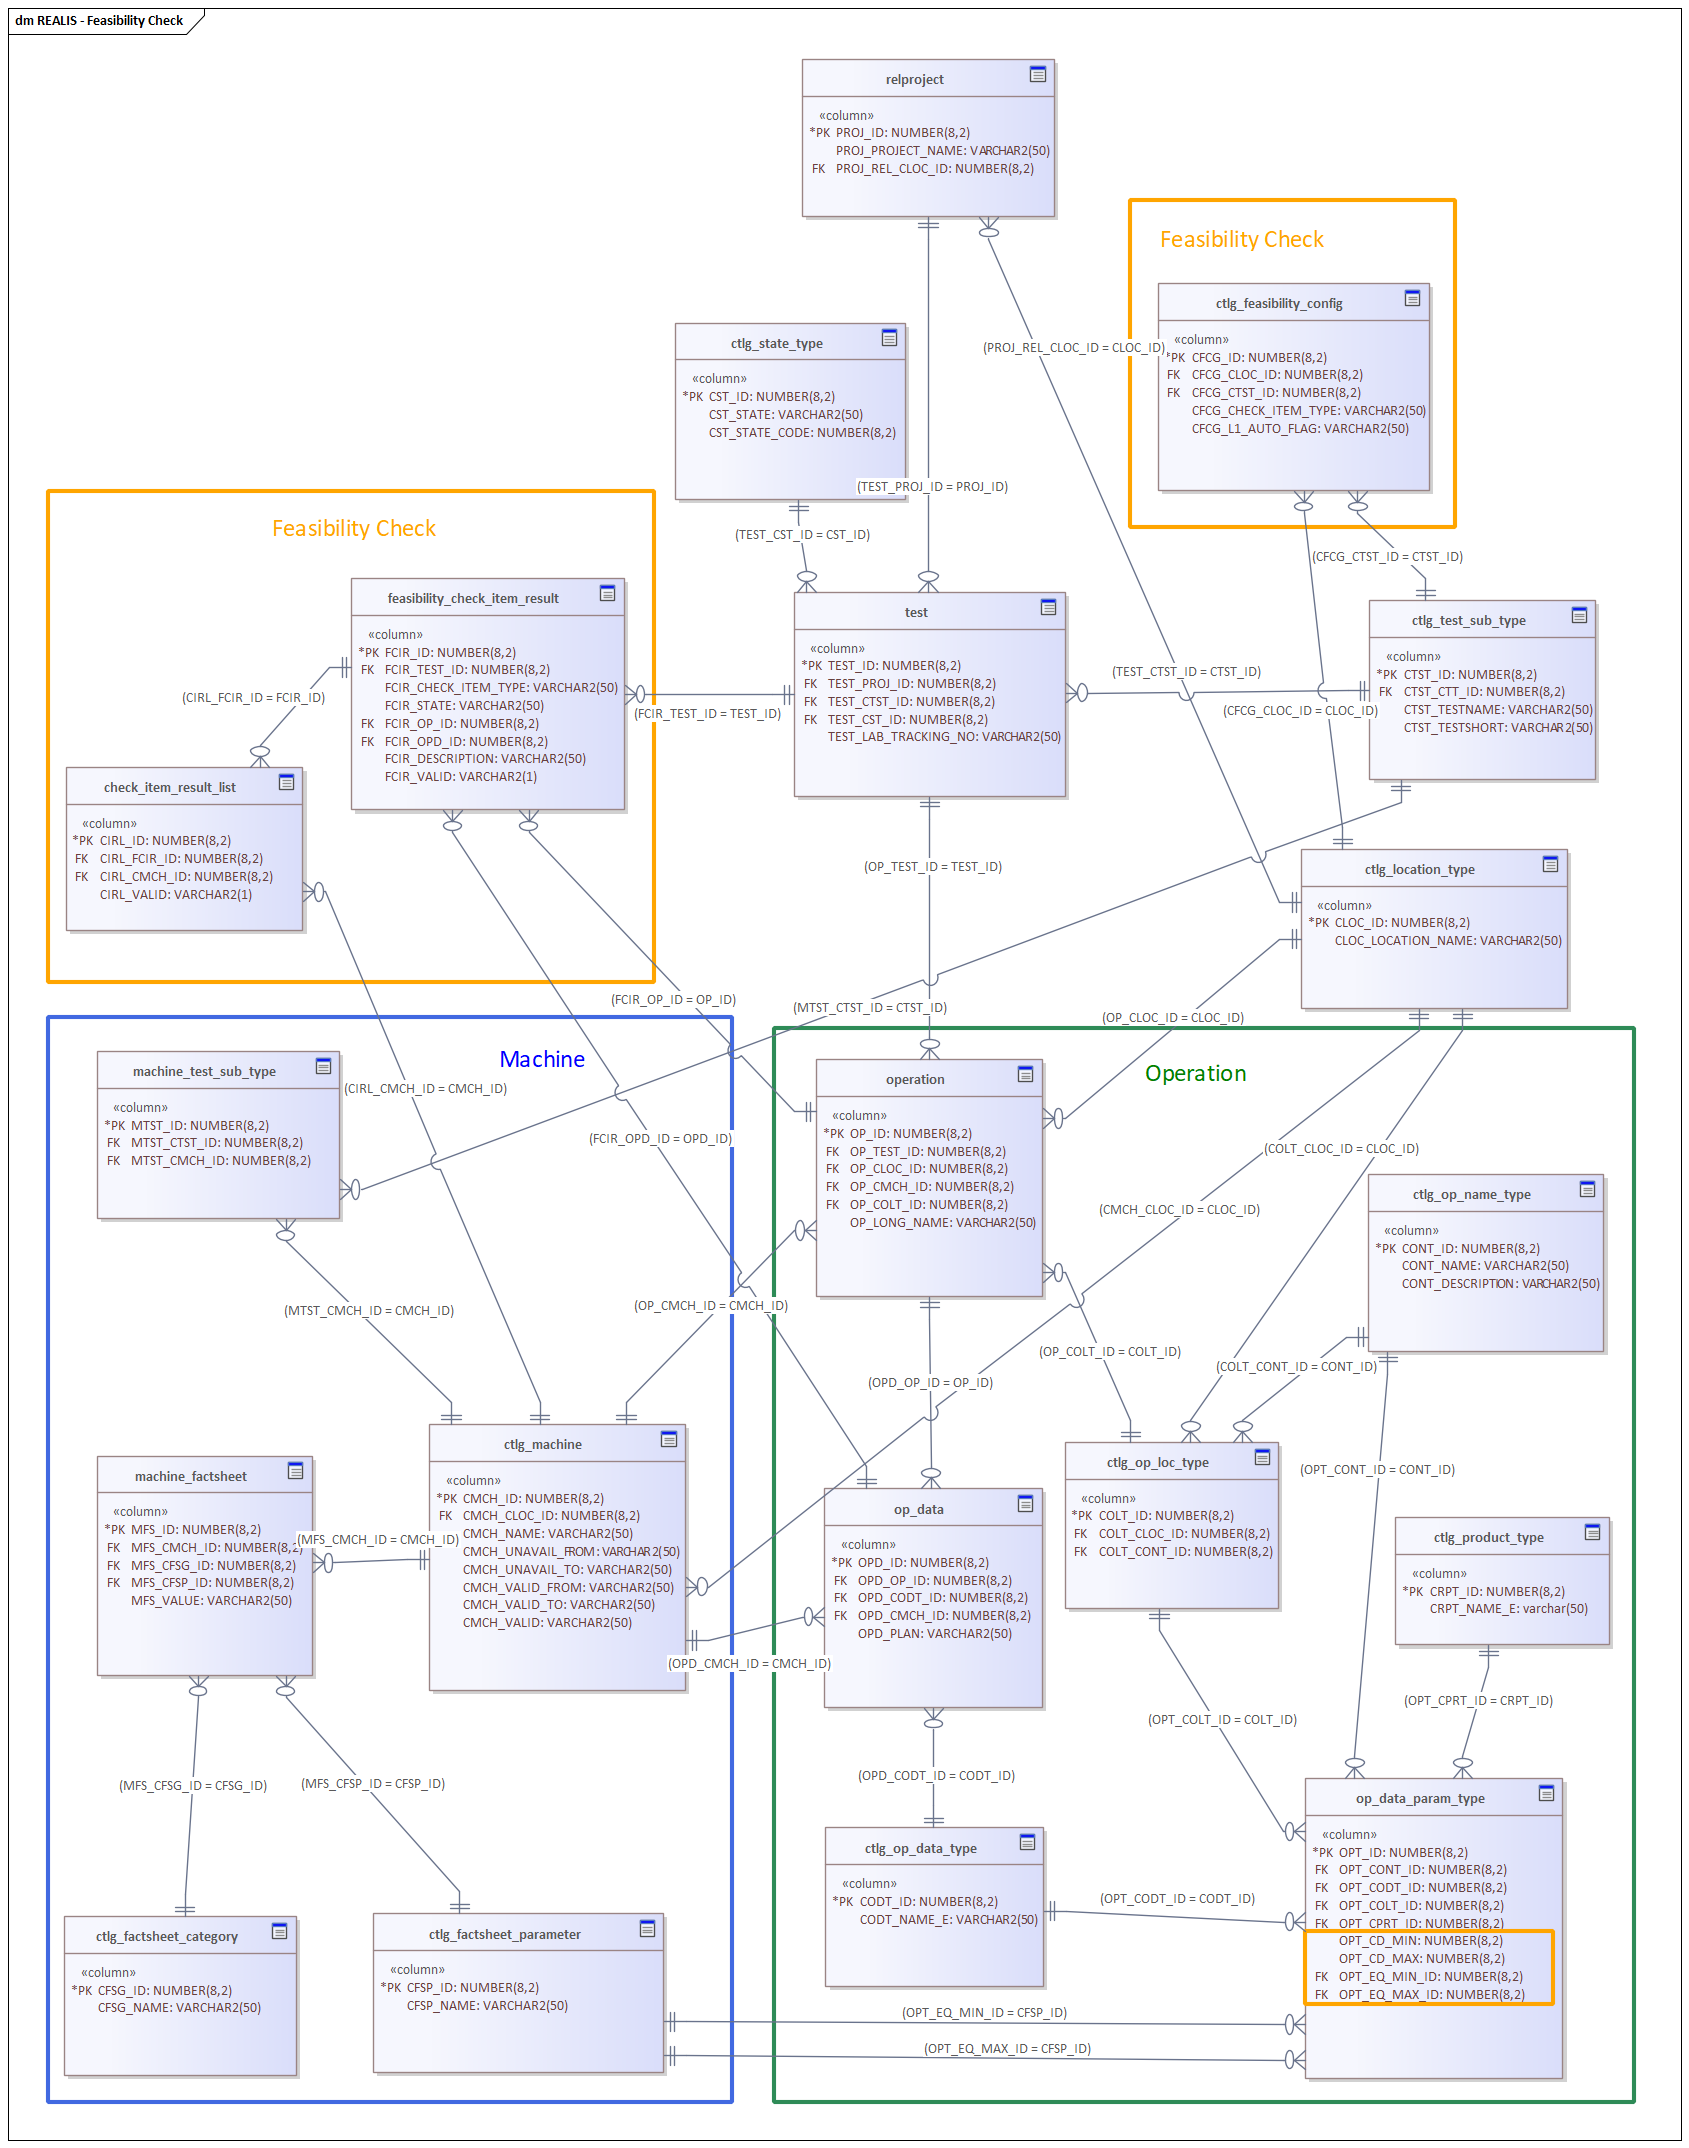
\includegraphics[width=0.98\paperwidth]{bilder/Datenbankdiagramm3.png}}
    \caption{REALIS Datenbankdesign}
    \label{fig:realis-datenbankdesign}
\end{figure}

Die Tabelle \texttt{ctlg\_op\_name\_type} bestimmt welche Arten von Operationen es gibt und legt indirekt über die Tabelle \texttt{ctlg\_op\_loc\_type} fest, welche Operations-Typen in welchen \gls{RPT}-Laboren verfügbar sind. Darüber hinaus definiert die 
\textbf{\texttt{op\_data\_\-param\_type}} Tabelle, welcher Parameter bei welcher Operation in welchem Labor für welche Produkttypen (\texttt{ctlg\_product\_type}) verfügbar ist. Hierbei sind das Labor und der Produkttyp aber nur optionale Einträge, um generische, laborübergreifende und/oder produktübergreifende Einträge zu ermöglichen.

Jeder (Stress-)Parameter einer Operation, der einen konkreten Wert definiert (\texttt{OPD\_\-PLAN}), muss von einer \textbf{Maschine} (\texttt{ctlg\_machine}) umgesetzt werden können. Die eng mit der Maschine verknüpften Tabellen befinden sich in der Abbildung \ref{fig:realis-datenbankdesign} im blau umrandeten Bereich. Eine Maschine ist verknüpft mit einem \textbf{Maschinen-Test-Typen} (\texttt{machine\_test\_sub\_type}), der die Maschine einem Test-Typen (\texttt{ctlg\_\-test\_\-sub\_type}) zuordnet. Des Weiteren besitzen Maschinen verschiedene \textbf{''Fact\-sheets''} (\texttt{machine\_factsheet}) mit einem \textbf{Parameter} (\texttt{ctlg\_\-factsheet\_\-para\-meter}) und einem Wert (\texttt{MFS\_VALUE}). Dieser Wert korrespondiert mit der PlanValue (\texttt{OPD\_\-PLAN}) des Operations-Parameters. 
Er gibt dabei ein Minimum oder ein Maximum der Maschine für diesen Parameter an. Deswegen gibt es (meist) für jeden Operations-Parameter-Typ zwei zugehörige Maschinen-Factsheet-Parameter(-Typen), die anhand ihres jeweiligen Wertes das Minimum und Maximum der Maschine für diesen Parameter festlegen.

Zur besseren Veranschaulichung ein konkretes Beispiel: Ein Temperaturtest besteht aus mehreren Operationen, darunter eine Stressoperation und eine anschließende Funktionsprüfung. Die Stressoperation enthält einen Temperatur-Parameter, dessen \texttt{OPD\_PLAN}-Wert die zu prüfende Testtemperatur definiert (z.B.: 100 °C). Gleichzeitig gibt es spezielle Temperatur-Stress-Maschinen, die über zwei Maschinen-Parameter verfügen: ''Temperatur-Min'' und ''Temperatur-Max''. Diese Parameter besitzen jeweils einen Wert (\texttt{MFS\_VALUE}) und legen darüber gemeinsam die Temperaturspanne fest, innerhalb der die Maschine arbeiten kann.


\subsection{Datenbankerweiterung für Feasibility Check}

Für die Durchführung des Feasibility Checks muss die Datenbank erweitert werden. Dabei sollen die in Kapitel \ref{Subsec:ParameterdestechnischenFeasibilityChecks} beschriebenen Parameter und die zugrunde liegende Logik umgesetzt werden. Zusätzlich müssen die Anforderungen aus Kapitel \ref{Chap:Anforderungen} berücksichtigt werden.

Der Feasibility Check bewertet den Parameter-Wert einer (Stress-)Operation in zwei Dimensionen. Die Überprüfung der \textbf{Sinnhaftigkeit} (\textbf{\gls{ConditionCheck}}) und die Überprüfung der \textbf{Durchführbarkeit} (\textbf{\gls{EquipmentCheck}}).
Dieser Parameter-Wert entspricht in der Datenbank REALIS dem Eintrag \textbf{\texttt{OPD\_PLAN}} in der Tabelle \texttt{op\_data}, die ihn definiert und den Parameter darstellt.

\textbf{\gls{ConditionCheck}} \\
Damit dieser Parameter-Wert auf Sinnhaftigkeit überprüft werden kann, werden in der generischen Verknüpfungs-Tabelle \texttt{op\_data\_param\_type} zwei neue Spalten hinzugefügt. Die Einträge definieren dabei den zulässigen bzw. ''sinnvollen'' Wertebereich für einen Parameter basierend auf den Faktoren: Operationstyp, Parametertyp, Labor und Produkttyp.

\setlength{\leftskip}{1em} 
\textbf{\texttt{OPT\_CD\_MIN}} - definiert die untere Grenze des zulässigen Wertebereichs

\textbf{\texttt{OPT\_CD\_MAX}} - legt die obere Grenze des zulässigen Wertebereichs fest

\setlength{\leftskip}{0em} 

\textbf{\gls{EquipmentCheck}} \\
Für den \gls{EquipmentCheck} wird ebenfalls die Tabelle \texttt{op\_data\_param\_type} um zwei Attribute ergänzt:

\setlength{\leftskip}{1em} 
\textbf{\texttt{OPT\_EQ\_MIN\_ID}} - Referenz auf den minimalen Maschinen-Parameter

\textbf{\texttt{OPT\_EQ\_MAX\_ID}} - Referenz auf den maximalen Maschinen-Parameter

\setlength{\leftskip}{0em} 

Die neuen Spalten dienen als Fremdschlüssel zu zwei Maschinen-Parametertypen (\texttt{ctlg\_factsheet\_parameter}) und ermöglichen die Zuordnung der passenden\linebreak Maschinen zu den jeweiligen Operations-Parametern. Die tatsächlichen Maschinen-\\Parameter-Werte stehen in der verknüpften \texttt{machine\_factsheet}-Tabelle im Feld\linebreak \texttt{MFS\-\_VALUE}. Dadurch lassen sich die Grenzen des umsetzbaren Wertebereichs aller Maschinen für einen spezifischen Operations-Parameter erfassen – eine Funktionalität, die im bisherigen Datenbankmodell von REALIS noch nicht gegeben war.


\textbf{Konfigurierbarkeit des automatisierten Feasibility Checks} \\
Die Konfigurierbarkeit des automatisierten Feasibility Checks legt fest, welche Tests automatisch geprüft werden und welche weiterhin manuell überprüft werden müssen, da manche Tests sich nicht für eine automatische eignen oder andere gar keine Feasibility Check Überprüfung benötigen.

 Dazu wird eine Konfigurationsmöglichkeit in der Datenbank geschaffen. Die Tabelle \textbf{\texttt{ctlg\_feasibility\_config}} ermöglicht die Festlegung, welche Tests automatisiert, manuell oder nicht geprüft werden müssen, abhängig von Labor(-Standort), Test-Typ und CheckItem(-Typ). Ein weiterer Vorteil dieser Konfiguration ist, dass der automatisierte Feasibility Check vor dem vollständigen ''Rollout'' getestet werden kann, indem er gezielt für bestimmte Tests aktiviert wird. Die Spalten der Datenbanktabelle sind in Tabelle \ref{tab:config-fields} erklärt.

\begin{table}[htbp]
    \centering
    \caption{Spalten der Feasibility Check Konfigurations-Tabelle: \texttt{ctlg\_\-feasibility\_\-config}}
    \footnotesize
    \renewcommand{\arraystretch}{1.2}
    \resizebox{\textwidth}{!}{ % Skaliert die Tabelle auf die Seitenbreite
    \begin{tabular}{p{0.3\linewidth} p{0.3\linewidth} p{0.35\linewidth}}
        \toprule
        \textbf{Feldname} & \textbf{Kurzbezeichnung} & \textbf{Beschreibung} \\
        \midrule
        \texttt{CFCG\_L1\_AUTO\_FLAG} & Automatisierungsstatus & Legt fest, ob ein Test automatisiert oder manuell durchgeführt werden soll. \\
        \midrule
        \texttt{CFCG\_CLOC\_ID} & Labor(-Standort) & Berücksichtigt das jeweilige Labor. \\
        \midrule
        \texttt{CFCG\_CTST\_ID} & Test-Typ & Differenzierung nach spezifischen Testarten. \\
        \midrule
        \texttt{CFCG\_CHECK\_ITEM\_TYPE} & CheckItem(-Typ) & Definiert, ob es sich um einen \gls{ConditionCheck} oder einen \gls{EquipmentCheck} handelt. \\
        \bottomrule
    \end{tabular}}
    \label{tab:config-fields}
\end{table}

Falls für eine bestimmte Kombination kein Eintrag in der Konfigurations-Tabelle existiert oder das Automatisierungsstatus-Flag auf \textit{null} gesetzt ist, impliziert dies, dass für diese Verknüpfung kein Feasibility Check erforderlich ist. Diese Regelung ist notwendig, da bestimmte Test-Typen oder Laborstandorte keinen Feasibility Check benötigen. Zudem können bei Einträgen auch die Felder Labor(-Standort), Test-Typ oder CheckItem(-Typ) auf \textit{null} gesetzt werden, um generische Definitionen zu ermöglichen und die Konfiguration flexibler zu gestalten.

\textbf{Speicherung der Feasibilitiy Check Ergebnisse} \\
Die (Teil-)Ergebnisse der durchgeführten Feasibility Checks werden in der Tabelle \textbf{\texttt{feasibility\_check\_item\_result}} gespeichert. Diese ist mit dem jeweiligen Test verknüpft und kann – sofern zutreffend – auch mit hierarchisch tieferliegenden, spezifischeren Ebenen wie der Operation oder einzelnen Parametern assoziiert werden. Diese Verknüpfungen sind jedoch optional, da in manchen Fällen bereits auf Test\-ebene eine abschließende Bewertung möglich ist oder der Test keine spezifischen Operationen und Parameter umfasst.

Jeder einzelne ''Teil-Check'' wird in Abhängigkeit vom jeweiligen CheckItem(-Typ) in der Tabelle abgelegt und umfasst unter anderem die Felder \texttt{FCIR\_STATE}, \texttt{FCIR\_\-DESCRIPTION} und \texttt{FCIR\_VALID}. Dabei dokumentiert \texttt{FCIR\_STATE} den Endstatus des jeweiligen ''Teil-Checks'' (siehe Kapitel \ref{Sec:Backend-Logik} und Abbildung \ref{tab:feasibility-states}), \texttt{FCIR\_DESCRIPTION} liefert eine benutzerfreundliche textuelle Begründung und \texttt{FCIR\_VALID} kennzeichnet, ob das Ergebnis aktuell gültig ist. Da ein Test mehrfach einem Feasibility Check unterzogen werden kann, werden bei jeder neuen Durchführung alle vorherigen Ergebnisse als ungültig markiert, verbleiben jedoch als Historie in der Datenbank.

Die in der Tabelle \texttt{feasibility\_check\_item\_result} gespeicherten Teil-Ergebnisse bilden somit die Grundlage für die Gesamtbewertung eines Tests. Das finale Feasi\-bility-Ergebnis wird aber nicht als einzelner Eintrag gespeichert, sondern durch die Aktualisierung des Teststatus repräsentiert. Anhand der aggregierten Teilergebnisse wird dem Test ein neuer Status zugewiesen: Scheitert mindestens einer der automatisierten ''Teil-Checks'' oder ist eine automatisierte Durchführung nicht möglich bzw. erlaubt, so erhält der Test den neu eingeführten Status ''\textbf{\texttt{MANUALFEASIBILITY}}'', welcher signalisiert, dass eine manuelle Überprüfung erforderlich ist. Werden alle ''Teil-Checks'' hingegen erfolgreich abgeschlossen, so wird der Test auf den bestehenden Status ''\textbf{\texttt{APPLY}}'' gesetzt und damit für den nächsten Schritt im Projekt-Lebenszyklus von REALIS freigegeben. Tritt ein Fehler auf oder bestehen andere Probleme, behält der Test den Status ''\textbf{\texttt{FEASIBILITYREQUESTED}}'', der unmittelbar nach dem Triggern des Feasibility Checks zugewiesen wird.

Wird der Equipment Check erfolgreich abgeschlossen, so werden zusätzlich die Maschinen, die die geforderten Parameter(-Werte) umsetzen können, in der Tabelle \textbf{\texttt{check\_item\-\_result\_list}} hinterlegt. Diese Tabelle stellt eine Verknüpfung zwischen den identifizierten Maschinen und dem entsprechenden Feasibility Check-Ergebnis her.

Durch diese Vorgehensweise wird sichergestellt, dass die detaillierten Teil-Ergeb\-nisse als Grundlage für die finale Testbewertung herangezogen werden, wodurch eine differenzierte und transparente Evaluation der Feasibility Checks möglich ist.





